\chapter{Modelo Criptográfico}

Demostraremos las garantías de seguridad de nuestro protocolo en el
\textit{framework Generalized Universal Composability} (GUC). GUC \cite{conf/tcc/CanettiDPW07}
es una generalizacion del \textit{framework Universal Composability}
\cite{conf/focs/Canetti01}. Ambos sirven para modelar protocolos criptgráficos concurrentes,
pero GUC adicionalmente modela protocolos concurrentes que comparten estado entre si.
Primero revisaremos el framework UC pues GUC se construye a partir de UC con pequeñas,
pero muy significativas, modificaciones.\\

\section{The Universal Composability framework (UC)}
\label{sect:uc}
UC es una metodología para modelar modularizadamente protocolos criptograficos que son ejecutados en redes
del ``mundo real" (por ejemplo internet). El espiritu de UC es diseñar un protocolo y luego abstraer la
seguridad que uno espera de él en un protocolo ideal, ejecutado en condiciones especiales que garantizan
su seguridad. Luego se debe demostrar que ejecutar el protcolo real y ejecutar el protocolo ideal es
escencialmente lo mismo, por lo tanto el protocolo real es tan seguro como el protocolo ideal.\\
Los protocolos reales son pueden ser ejecutados concurrentemente con muchos otros protocolos,
y tambien pueden ser ejecutados distribuidos entre varios participantes.
Como en el mundo real el protocolo puede ser monitoreado por terceros y algunos participantes pueden salirse
arbitrareamente del protocolo atentando con la seguridad. Todo el posible mal comoportamiento es ejecutado por una sola
máquina, el Adversario (real) $\mathcal{A}$. En una ejecución del protocolo el adversario puede espíar y
manipular todos los mensajes intercambiados, también puede manejar la distribución de mensajes a su antojo,
y además puede \textit{corromper} participantes del protocolo y ejecutar codigo arbitrario en ellos.\\
Por otro lado estan los protocolos ideales, llamados \textit{funcionalidades ideales} denotadas por 
$\mathcal{F}$. Las funcionlidades ideales son ejecutadas en un mundo ideal, donde es una entidad confiable
la encargada de ejecutar su código. En el mundo ideal existe un adversario ideal o \textit{simulador}
$\mathcal{S}$, pero este no puede espíar ni controlar la comunicación más de lo que la funcionalidad ideal
permite.\\
La configuración en la que el protocolo real es ejecutado con el adversario real es conocida como \textit{mundo
real}, y la configuración en que la funcionalidad ideal es ejecutada con el adversario ideal es conocida como
\textit{mundo ideal}. En ambos mundos la ejecución del protocolo concurrentemente con otros protocolos esta a cargo
de una máquina especial conocida como el ambiente y denotado por $\mathcal{Z}$. De este modo en UC los protocolos
pueden ser analizados aislados de resto del mundo. Para asegurarse que el protcolo real alcanza la seguridad deseada
se debe tener que para cualquier ejecución del protocolo en el mundo real y para cualquier estrategia adversarial
(esto es para todo ambiente y para todo adversario) existe una estrategia adversarial con recursos limitados (un
adversario ideal) que tiene el mismo efecto que la estrategia adversarial real (el ambiento no es capaz de percatarse
de ninguna diferencia entre la ejecución del protocolo real y el protocolo ideal).\\
Para definir formalmente las nocienes intuitivas descritas anteriormente es necesario introducir un modelo de
cálculo conocido como Máquinda de Turing Interactiva , más precisamente sitemas de ITM.

\subsection{Sistemas de Máquinas de Turing Interactivas}

Las Máquinas de Turing Interactivas corresponden a Máquinas de Turing con cintas especiales que pueden ser
escritas externamente. A dichas cintas las llamamos escribibles externamente (EW), y son de escritura única,
es decir, el cabezal siempre se mueve a la derecha.

\begin{definicion}
Una Máquina de Turing Interactiva $M$ es una Máquina de Turing con las siguientes cintas:
\begin{enumerate}
    \item Una cinta EW de identidad.
    \item Una cinta EW del parámetro de seguridad.
    \item Una cinta EW de entrada.
    \item Una cinta EW de comunicación entrante.
    \item Una cinta EW de salidas de subrutinas.
    \item Una cinta de salida.
    \item Una cinta de bits aleatorios.
    \item Una cinta de activación, de lectura y escritura y de 1 bit de tamaño.
    \item Una cinta de lectura y escritura para trabajo. 
\end{enumerate}
\end{definicion}

La cinta de identidad contiene un string que representa la identidad de $M$, que se interpreta
como si estuviera compuesto por dos substrings: el identificadod de sesión (SID) y el identificador
de participante (PID). Identificamos a cada instancia de una ITM (ITI) por el par
$\mu = (\langle M \rangle, id)$, con $\langle M \rangle$ el código de $M$ y $id$ el contenido de la cinta
de identidad. En general omitimos los $\langle \rangle$ y con $M$ nos referimos tanto a la máquina como
al código.\\
La cinta del parámetro de seguridad contiene un string de la forma $1^k$, con $k$ el parámetro de seguridad 
\footnote{El parámetro de seguridad indica el nivel de seguridad en el cual se esta ejecutando
la máquina, y en general mientras crece se debería tener que la seguridad del protocolo ejecutado
con la máquina también crece.}.\\
La cinta de salida contendrá la salida de $M$ una vez que haya terminado.\\
La cinta de bits aleatorios contiene suficientes bits aleatorios para que $M$ pueda realizar sus cálculos.\\
La cinta de trabajo es la usual cinta de trabajo de las Máquinas de Turing.\\
La cinta de activación tiene el valor 0 si la $M$ no esta activada y 1 si lo esta. La secuencia de
configuraciones de una ejecución de $M$
\footnote{Una configuración corresponde a un objeto que determina completamente un instante
en la computación de una MT. Podemos ver la ejecuciónde una MT como una secuencía de configuraciones, donde la
primera configuración corresponde a la MT en su estado inicial y la(s) cinta(s) con la(s) entrada(s), y la
configuración final corresponde a la MT en un estado final.}
esta compuesta por subsecuencias en las
que en cada configuración la $M$ esta activada. A dichas subsecuencias se les conoce como \textit{secuencias
de activación}.\\
Las otras cintas toman importancia cuando $M$ es ejecutada ``conectada" con otras máquina
en un Sistema de ITMs (sITM).\\

\begin{definicion}
Un Sistema de ITMs $S$ viene dado por $S = (I, C)$, donde $I$ es la ITM inicial y $C$ es la función
de control $C:\{0,1\}^* \to \{0,1\}$.
\end{definicion}
Inicialmente la ITI $\mu_0 = (I, 0)$ es activada, el sITM terminará cuando $I$ termine y su
salida sera lo que $I$ deje en su cinta de salida.\\
Una ITI $\mu = (M, id)$ puede escribir en una de las cintas de otra ITI $\mu' = (M', id')$, 
para ello es necesario que $\mu$ ejecute una instrucción
especial llamada \texttt{escritura-externa} y debe especificar la cinta en de $\mu'$ en la que quiere
escribir y los datos a escribir en esa cinta
\footnote{Formalmente podríamos decir que $M$ entra en un estado especial y en su cinta de
trabajo se encuentra un string $x$ que determina $\mu'$, la cinta objetivo y los datos a escribir
en la cinta objetivo}.
La semántica de la instrucción de \texttt{escritura-externa} es como sigue:\\

\begin{enumerate}
    \item Si la funciónde control $C$ aplicada a toda la secuencia de intrucciones \texttt{escritura-externa}
          que se han realizado hasta ahora retorna 0, entonces la instrucción es ignorada.
    \item Si $C$ retorna 1 pero no existe una ITI en el sITM $\mu'' = (M'', id'')$ talque $id''=id'$, se
          crea una nueva ITI con código $M'$ y con identidad $id'$. Para ello se crea una nueva ITM
          que en la cinta de identidad contiene $id'$, el la cinta del parámetro de sugirdad contiene $1^k$
          y en la cinta de bits aleatorios contiene suficientes bits aleatorios. A continuación se evalúa
          el punto siguiente.
    \item Si $C$ retorna 1 y existe una ITI en el sITM $\mu'' = (M'', id'')$ talque $id''=id'$:
    \begin{enumerate}
        \item Si la cinta objetivo de la intrucción era la cinta de comunicación entrante de $\mu'$, entonces
              los datos especificados son escritos en la cinta de comunicación entrante de $\mu''$ y $\mu''$
              es activada. Notemos que esto es hecho independiente de si el código de $\mu''$ es el mismo
              código especificado por $\mu$, con el fin de rescatar que una ITI no conoce el código de la
              ITI con que se comunica a través de escrituras en la cinta de comunicación entrante.
        \item Si la cinta objetivo era la cinta de entrada de $\mu'$ y $M' = M''$, entonces los datos
              especificados son escritos en la cinta de entrada de $\mu''$ y $\mu''$ es activada. En este caso
              la instrucción modela llamados a otras ITIs como subrutina, dentro de un entorno seguro ($\mu$
              conoce el código que esta ejecutando $\mu''$).
        \item Si la cinta objetivo es la cinta de salida de subrutina de $\mu'$, entonces los datos
              especificados son escritos en la cinta de salida de subrutina de $\mu''$. En este caso la
              instrucción modela el retorno de una llamada a subrutina, en que la subrutina no conoce
              el código de la ITI que la llamó.
    \end{enumerate}
\end{enumerate}

Adicionalmente consideramos funciones de control \textit{extendidas} las cuales, además de permitir
o no permitir instrucciones \texttt{escritura-externa}, son capaces de traducir una intrucción de
\texttt{escritura-externa} en otra. Por ejemplo, una función de control extendida puede obligar
a que todas las ITM creadas tengan un código preespecificado $M$ traduciendo cualquir instrucción
\texttt{escritura-externa} con código $N$ a una instrucción de \texttt{escritura-externa} con código
$M$. Los sITM con función de control extendida los llamaremos sITM extendidos.\\

Como veremos más adelante, nos interesará especialmente la salida de un sITM.

\begin{definicion}
Denotamos a la variable aleatoria obtenida al ejecutar el sITM $(I,C)$ con parámetro de seguridad $k$, entrada $x$
y escogiendo los bits aleatorios necesarios para su ejecución al azar por $\mathrm{OUT}_{(I,C)}(k, x)$.
$\mathrm{OUT}_{(I,C)}$ denota a la familia de variables aleatorias\\
$\{\mathrm{OUT}_{(I,C)}(k, x)\}_{k\in\mathbb{N}, x\in\{0,1\}^*}$.
\end{definicion}

Como es usual nos limitaremos a sITMs ``eficientes", es decir el tiempo completo
de ejecución esta acotado por $p(|x| + k)$, con $p$ un polinomio. Se puede garantizar que un sITM $(I, C)$ es
eficiente si la ITM inicial es una PPT (del inglés \textit{Probabilistic Polynomial time Turing machine}).

\begin{definicion}
Sea $p:\mathbb{N} \to \mathbb{N}$. Decimos que una ITM $M$ esta localmente $p-acotada$ si, en cualquier punto
de su ejecución, el numero total de pasos tomados por $M$ es a lo más $p(n)$, donde
$$n = k + n_I - n_O - k\cdot n_N,$$
$k$ es el parámetro de seguridad, $n_I$ es el numero total de bits escritos en la cinta de entrada de $M$,
$n_O$ es el numero total de bits escritos por $M$ a otras ITMs, y $n_N$ es el número total de otras ITMs
en las que $M$ escribe.
\end{definicion}

\begin{definicion}
Si una ITM $M$ esta localmente $p-acotada$ y además $M$ solo escribe en ITMs localmente $p-acotadas$, entonces
decimos que $M$ es $p-acotada$.
\end{definicion}

\begin{definicion}
Una ITM $M$ es una PPT si existe un polinomio $p$ talque $M$ es $p-acotada$.
\end{definicion}

\subsection{Ejecución de un protocolo}

Definamos primero qué es un protocolo y una instancia de un protocolo.

\begin{definicion}[Protocolo PPT]
Un protocolo PPT (o simplemente protocolo) $\pi$ es la PPT que contiene el código a ejecutar por cada
participante del protocolo.
\end{definicion}

\begin{definicion}[Instancia de un protocolo]
Dado un sITM $S$, una instancia de un protocolo $\pi$ con SID $sid$ es el conjunto de ITIs
cuyo código es $\pi$ y cuyo SID es $sid$.
\end{definicion}

\begin{definicion}[Participante]
Una ITI $\mu$ es un participante de una instancia de $\pi$ con SID $sid$ si el SID de $\mu$ es $sid$.
\end{definicion}

\begin{definicion}[Sub-participante]
Una ITI $\mu$ es sub-participante de una sesión del protcolo $\pi$ si algun participante o sub-participante
de de la sesión de $\pi$ escribe en la cinta de comunicación entrante o en la cinta de input de $\mu$.
\end{definicion}

La ejecución de un protocolo en UC está parametrizada por tres ITMs:

\begin{itemize}
    \item El protocolo a ser ejecutado $\pi$.
    \item El ambiente $\mathcal{Z}$.
    \item El adversario $\mathcal{A}$ (o $\mathcal{S}$).
\end{itemize}

Con las tres ITMs construimos el sITM  extendido $(\mathcal{Z}, C^{\pi, \mathcal{A}}_\mathrm{EXEC})$.
La función de control $C^{\pi, \mathcal{A}}_\mathrm{EXEC}$ basicamente se encarga de que la primera ITM
invocada por $\mathcal{Z}$ sea $\mathcal{A}$, y de que $\mathcal{Z}$ solo invoque ITMs con código $\pi$ y
SID fijo. En la figura \ref{func_control} se detalla su funcionamiento.

\begin{figure}
\begin{centering}
\framebox{\begin{minipage}[t]{1\columnwidth}
La función de control $C^{\pi, \mathcal{A}}_\mathrm{EXEC}$  ejecutada con ambiente $\mathcal{Z}$,
adversario $\mathcal{A}$ y protocolo $\pi$ procede como sigue:
\begin{enumerate}
    \item Para el ambiente $\mathcal{Z}$:
    \begin{enumerate}
        \item El código de la primera instrucción \texttt{escritura-externa}
              es cambiado por el código de $\mathcal{A}$.
        \item Para cualquier otra instrucción \texttt{escritura-externa},
              si la ITI objetivo es distinta de $\mathcal{A}$ entonces cambiar el código por $\pi$.
    \end{enumerate}
    \item Para el adversario $\mathcal{A}$:
    \begin{enumerate}
        \item asdasd
    \end{enumerate}
    \item Suppose $(M_{j}, \mathtt{Run})$ is received from $\mathcal{C_I}$. Set
          $J_M \leftarrow J_M \cup \{j\}$. If $|J_M | \geq k/2$, then sort the list $L$ lexicographically
          to form a list $L'$, and hand
          $((\mathcal{S}, M_{j}, \mathtt{Output}, L'), \{M_l , \mathtt{Output}, L'\}_{l=1}^{k})$ to
          to $\mathcal{C_I}$. Otherwise, hand $\mathcal{C_I}$ the list $(\mathcal{S}, M_{j}, \mathtt{Run})$
\end{enumerate}
\end{minipage}}
\end{centering}
\caption{La función de control $C^{\pi, \mathcal{A}}_\mathrm{EXEC}$}
\label{func_control}
\end{figure}

Denotamos la salida de la ejecución de un protocolo $\pi$ en UC por
$\mathrm{EXEC}_{\mathcal{Z}, \mathcal{A}, \pi} = \mathrm{OUT}_{(\mathcal{Z}, C^{\pi, \mathcal{A}}_\mathrm{EXEC})}$

\begin{figure}[hp]
    \centering
    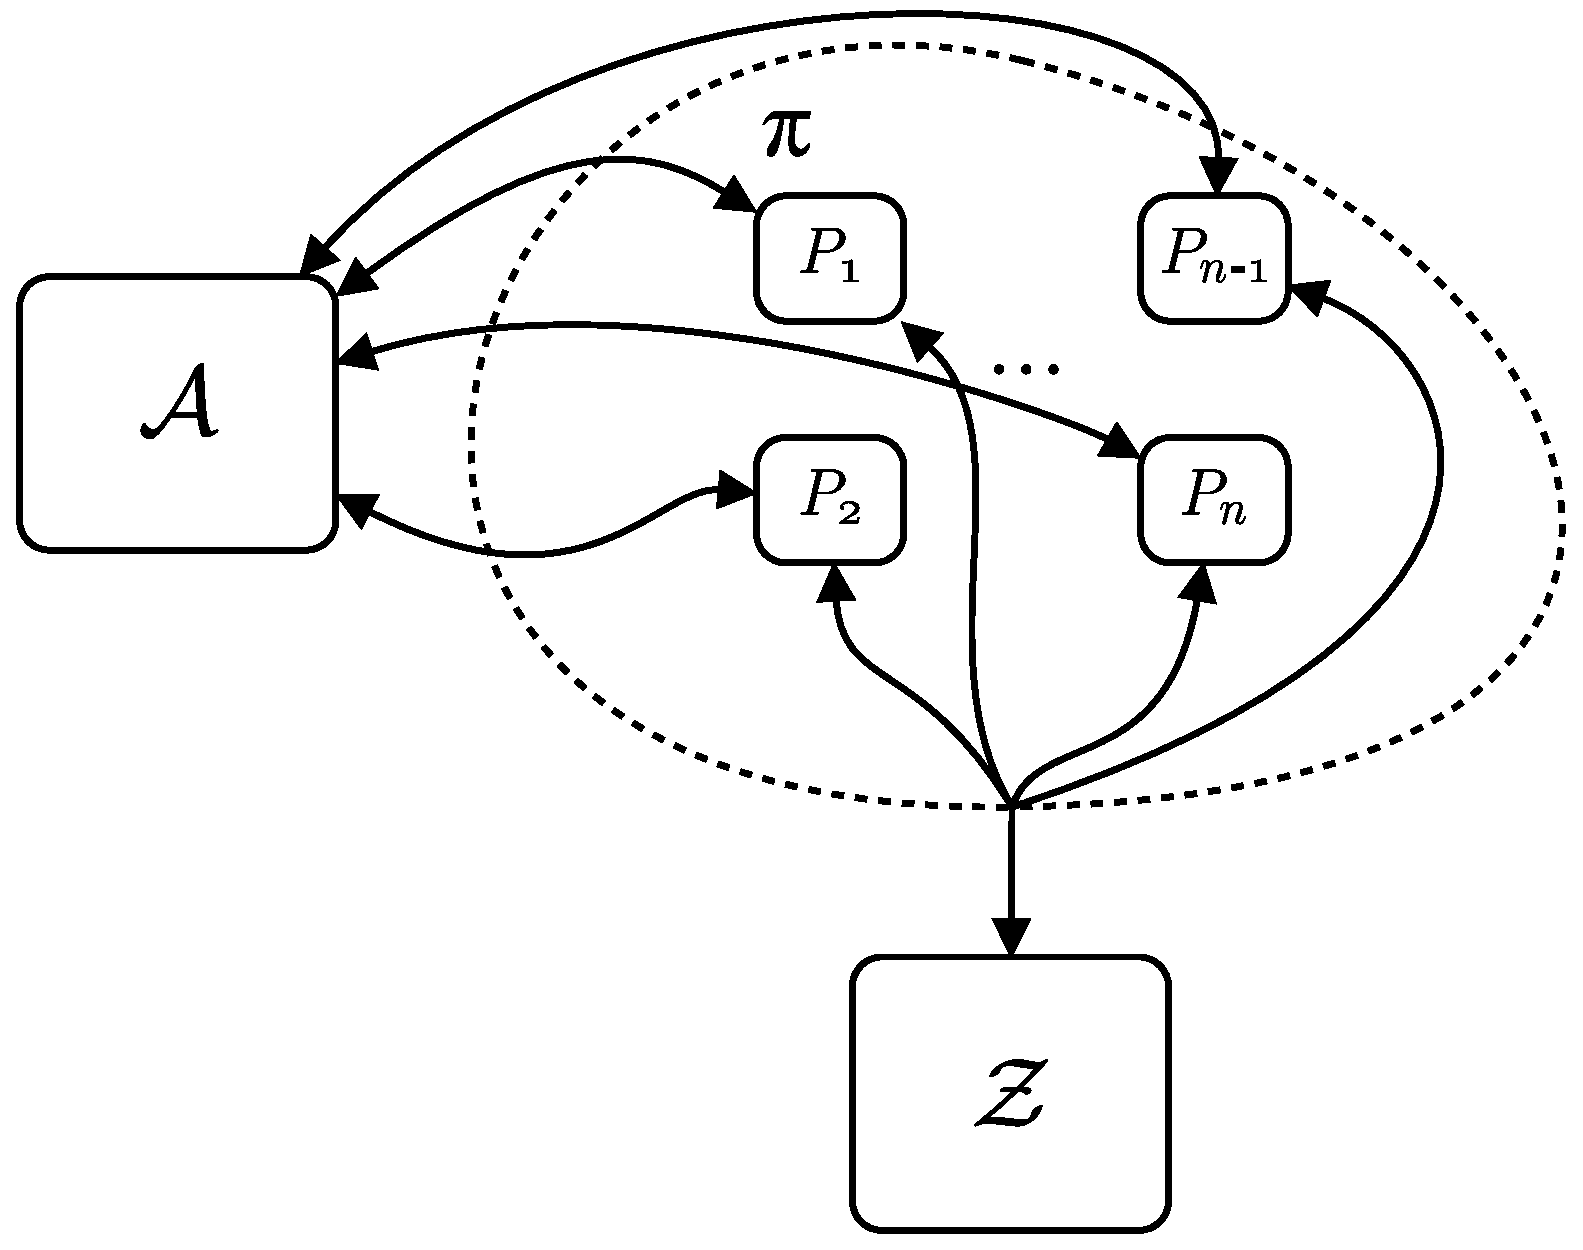
\includegraphics[width=0.6\textwidth]{figs/mundo_real}
    \caption{Ejecución de un protocolo en UC}
    \label{fig:mundo_real}
\end{figure}

\subsection{Teorema de composición}

La noción principal que entrega UC es la emulación de protocolos, que viene dada por la inabilidad de
$\mathcal{Z}$ de distinguir entre la ejecución de dos protocolos.

\begin{definicion}
Decimos que un protocolo $\pi$ UC-emula a otro procotolo $\phi$ si y solo si para cualquier ambiente
$\mathcal{Z}$ y para cualquier adversario $\mathcal{A}$ existe un adversario $\mathcal{S}$ talque
$$\mathrm{EXEC}_{\mathcal{Z}, \mathcal{A}, \pi} \approx \mathrm{EXEC}_{\mathcal{Z}, \mathcal{S}, \phi}$$
\end{definicion}

Supongamos que tenemos un protocolo $\pi$, que llama como subrutina a $\rho$. Si ningun ambiente puede
distinguir entre la ejecución del protocolo $\rho$ de otro protocolo $\phi$, es útil preguntarse si se pueden
cambir todas las llamadas de $\pi$ a $\rho$ por llamadas a $\phi$ sin cambiar el funcionamiento de
$\pi$. La conjetura anterior es corroborada por el teorema \ref{teo:composicion}, el teorema de composición.
Definamos primero que es ``cambiar todas las llamadas a $\rho$ por llamadas a $\phi$".

\begin{definicion}[Operador Composicion]
Sea $\pi$ un protocolo que (posiblemente) hace llamadas a $\rho$. Definimos el operador composición $/$ de forma tal
que $\pi^{\rho/\phi}$ es identico que el protocolo $\pi$ salvo que cada instrucción \texttt{escritura-externa}
con código $\rho$, es cambiada por la misma instrucción \texttt{escritura-externa} con código $\phi$.
\end{definicion}

Una propiedad adicional que necesitan cumplir los protocolos es que sean \textit{soubroutine respecting}, que
basicamente significa que no comparten estado.

\begin{definicion}[Protocolo soubroutine respecting]
Decimos que un protocolo $\rho$ es soubroutine respecting si ningún participante o sub-participante de $\rho$
pasa input o recibe output de una ITI que es participante o sub-participante de otra instancia de algun
protocolo.
\end{definicion}

\begin{teorema}[Composición]
Sean $\pi, \rho, \phi$ protocolos tales que $\rho$ UC-emula a $\phi$ y $\rho$ y $\phi$ son protocolos
soubroutine respecting. Entonces el protocolo $\pi^{\rho/\phi}$ UC-emula al protoclo $\pi$.
\label{teo:composicion}
\end{teorema}

La demostración del teorema \ref{teo:composicion} se puede encontrar en \cite{UC:completo}, a continuación
mostramos intuitivamente porque el teorema se debería cumplir.\\
Notemos que el protocolo $\pi$ puede invocar una cantidad indeterminada de protocolos
que se pueden ejecutar concurrentemente
con con $\rho$. Es precisamente por eso que $\pi^{\rho/\phi}$ podría no UC-emular a $\pi$, pues en la configuración
en la cual es ejecutado $\phi$, donde ningún ambiente puede distinguirlo de $\rho$, se ejecuta solamente una
instancia de $\phi$ y de ningún otro protocolo más. Lo que permite concluir acerca de $\pi^{\phi/\rho}$ es la
cuantificación sobre todos los ambientes y que tanto $\rho$ como $\phi$ son protocolos \textit{soubroutine
respecting}. Al cuantificar sobre todos los ambientes estamos diciendo que, en particular, la UC-emulación
también se tiene para ambientes que simulan internamente ejecuciones de otros protocolos como las que podría
hacer $\pi$. El único problema podría ser que las ejecuciones en paralelo de otros protocolos esten
``correlacionadas'' de alguna forma con $\rho$, pero esto no es posible pues al ser $\rho$ \textit{soubroutine respecting}
su ejecución es independiente de cualquier otro protocolo. Dicho de otra forma, para que un protocolo
este ``correlacionado'' con $\rho$ es necesario que $\rho$ lo llame directamente, o que ambos llamen a un protocolo
en común. El primer caso no es problemático, pues el protocolo correlacionado seria un subprotocolo de $\rho$
y sería parte de una ejecucion de $\rho$. El segundo caso no es posible, pues el protocolo que $\rho$ compartiría
sería una instancia externa y contradeciría que $\rho$ es \textit{soubroutine respecting}.\\

Otra forma de interpretar el teorema de composición es que nos permite asumir que el protocolo $\pi$ hace llamadas
a $\phi$ y no a $\rho$, lo cual puede ser útil cuando no sabemos si $\rho$ es seguro pero asumimos que $\phi$
si lo es. En tal caso $\phi$ sería una \textit{funcionalidad ideal}.

\subsection{Funcionalidades Ideales}
Para definir la seguridad de un protocolo en UC es necesario diseñar una funcionalidad ejecutada por una entidad
confiable en un protocolo que consideramos seguro. A la funcionalidad se le llama \textit{funcionalidad ideal} y
generalmente se le denota por la letra $\mathcal{F}$. Al protocolo se le llama \textit{protocolo ideal} y se
denota por $\mathrm{IDEAL}_\mathcal{F}$.Todo el cómputo del protocolo es realizado por $\mathcal{F}$, pues
los participantes solo ejecutan el código del \textit{participante tontito}

\begin{definicion}[Participante tontito]
Una instancia del participante tontito, denotado por $\tilde P$, es una ITI cuyo código es el siguiente:
\begin{enumerate}
    \item Si recibe $m,$ escribe $m$ en cinta de entrada de la funcionalidad $\mathcal{F}$.
    \item Si $\mathcal{F}$ retorna $m$, escribe $m$ en su cinta de output. 
\end{enumerate}
\end{definicion}

La funcionalidad ideal recibirá entradas de los participantes tontitos y escribira en su cinta de salida de
subrutina los resultados del cómputo que corresponden a cada particpante. Por lo tanto su funcionamiento
entrada/salida debe ser el deseado, esto es la funcionalidad debe ser \textit{correcta}. Adicionalmente
debe rebelar solo la información necesaria, de modo tal que la consideremos \textit{segura}. Una ITI
que ejecuta el código de una funcionalidad ideal sera creada igual que cualquier otra ITI, a excepción
que su cinta de identiadad tendrá como contenido un string de la forma $sid||\perp$, de modo tal que $\perp$
es un símbolo especial distinto a cualquier otro PID.\\
Como en una instancia del protocolo $\mathrm{IDEAL}_\mathcal{F}$ la comunicación entre participantes y
funcionalidades (y de este modo entre participantes) es por la cinta de entrada y la cinta de salida
de subrutina, el adversario del protocolo ideal $\mathcal{S}$ se vé límitado en su capacidad de
espiar o modificar la comunicación. En primera instancia $\mathcal{S}$  no tiene ninguna injerencia en
la comunicación, pero en general para que $\mathrm{IDEAL}_\mathcal{F}$ sea un protocolo ``implementable''
por un protocolo real es necesario que $\mathcal{F}$ de cierta injerencia a $\mathcal{S}$ en la comunicación.
En general se asume que las respuestas de $\mathcal{F}$ a los participantes tontitos pueden ser retradas tanto
como $\mathcal{S}$ lo desee, incluso por un tiempo infinito. El filtraje de información dependera del propósito
de $\mathcal{F}$.\\
De forma simular a la UC-emulación definimos la UC-realización de una funcionalidad ideal.

\begin{definicion}[UC-realización]
Decimos que un protocolo $\pi$ UC-realiza a la funcionalidad ideal $\mathcal{F}$ si para todo ambiente
$\mathcal{Z}$ y para todo adversario real $\mathcal{A}$ existe un adversario ideal $\mathcal{S}$ talque
$$
\mathrm{EXEC}_{
    \mathcal{Z},
    \mathcal{A},
    \pi}
\approx
\mathrm{EXEC}_{
    \mathcal{Z},
    \mathcal{S},
    \mathrm{IDEAL}_\mathcal{F}}
$$
\end{definicion}

Como corolario del teorema \ref{teo:composicion} tenemos el siguiente resultado.

\begin{corolario}
Sean $\pi, \rho$ protocolos y $\mathcal{F}$ una funcionalidad ideal tales que $\rho$ UC-realiza
$\mathcal{F}$ y $\rho$ es un protocolo soubroutine respecting. Entonces el protocolo
$\pi^{\rho/\mathrm{IDEAL}_\mathcal{F}}$ UC-emula a $\pi$.
\label{corolario:uc-realizacion}
\end{corolario}

\begin{figure}[hp]
    \centering
    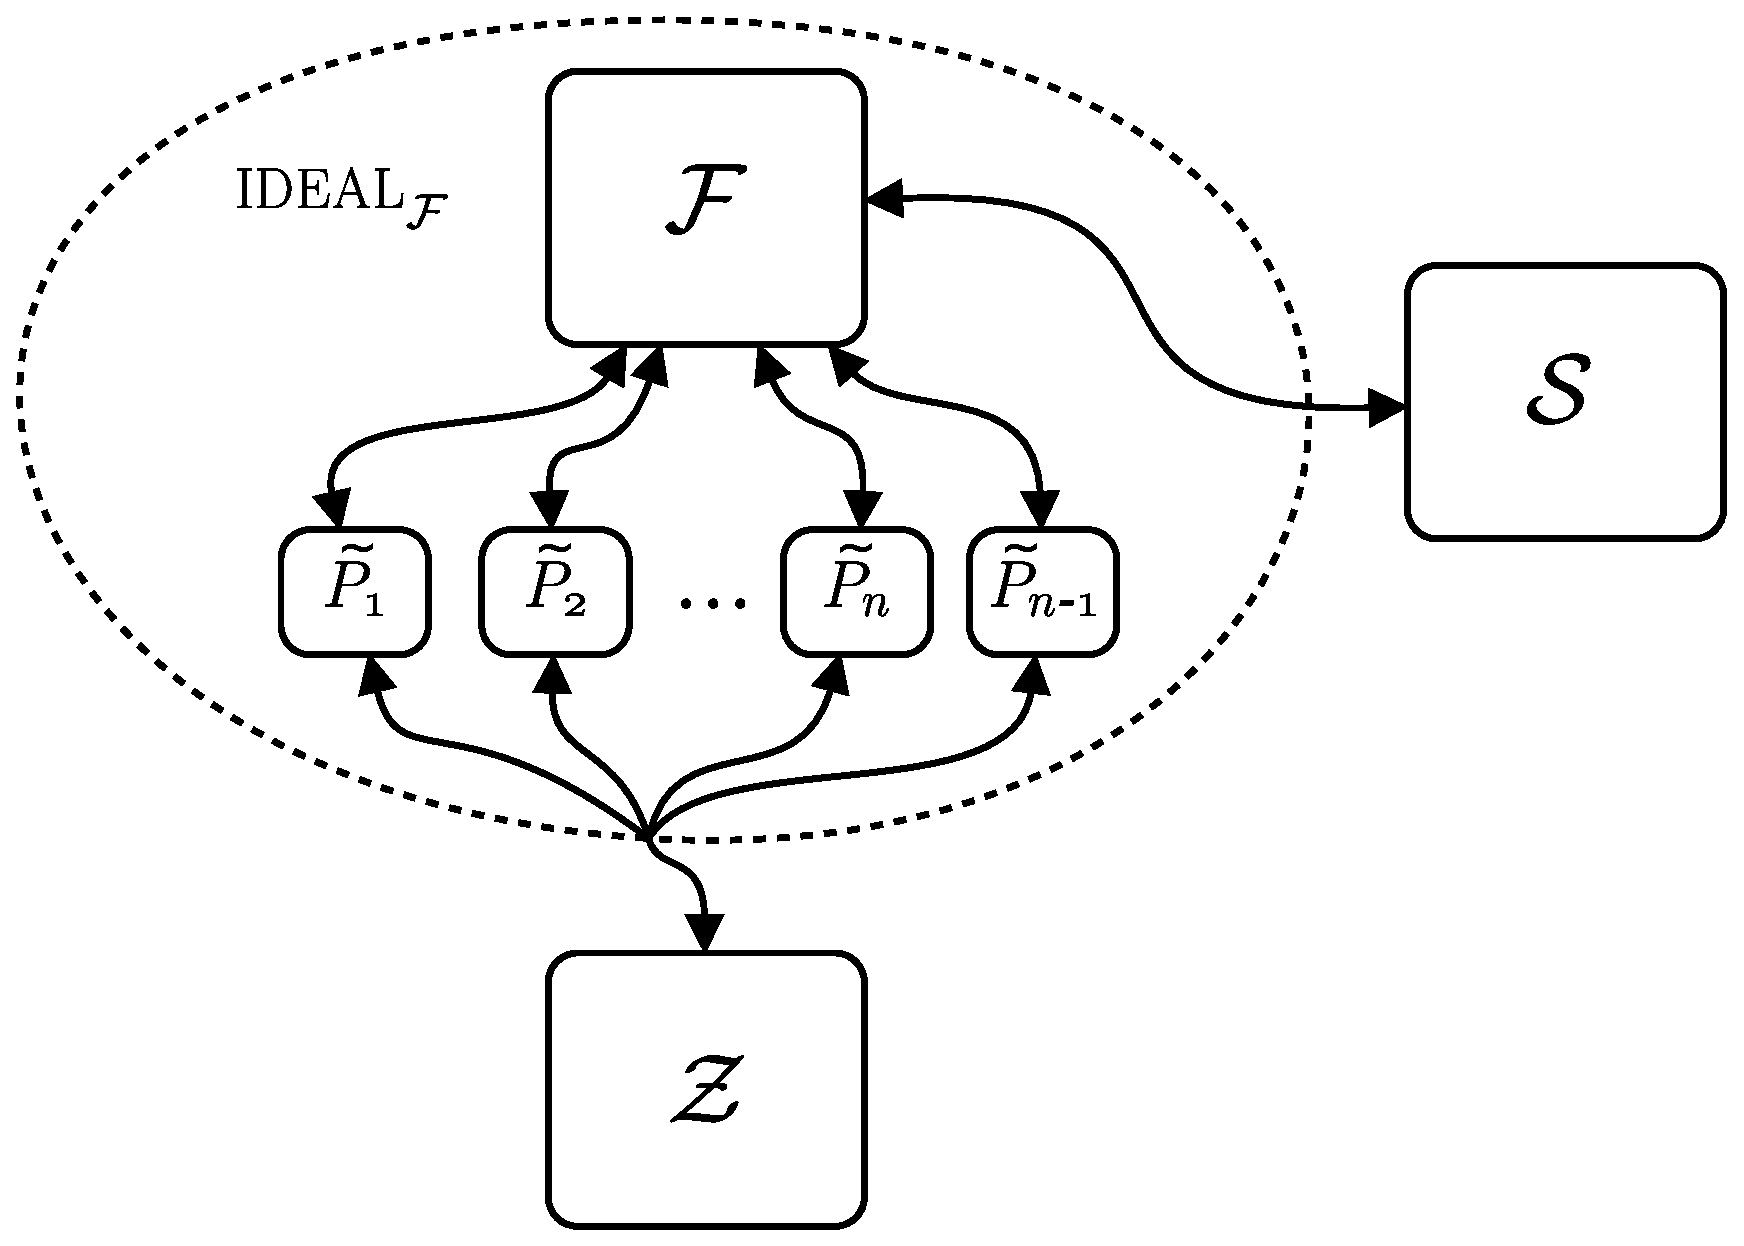
\includegraphics[width=0.7\textwidth]{figs/mundo_ideal}
    \caption{Ejecución del protocolo $\mathrm{IDEAL}_\mathcal{F}$ en UC}
    \label{fig:mundo_ideal}
\end{figure}

El corolario \ref{corolario:uc-realizacion} es lo que le da sentido a la ``metodología'' de UC,
conocida como el método de Dolev-Yao \cite{dolev_yao}, pues permite diseñar y probar la seguridad
de protocolos criptográficos complejos de forma modularizada, al introducir los \textit{modelos
híbridos}.

\begin{definicion}[Modelo Híbrido]
Decimos que un protocolo $\pi$ es ejecutado en el modelo $\mathcal{F}$-híbrido si cada participante puede
hacer llamados a una instania local al protocolo $\pi$ función ideal $\mathcal{F}$. 
\end{definicion}

De forma similar se puede definir el modelo $\mathcal{F}_1, \ldots, \mathcal{F}_n$-híbrido para
funcionalidades ideales $\mathcal{F}_1, \ldots, \mathcal{F}_n$.\\

En la figura \ref{fig:dolev-yao} se puede apreciar la forma de analizar en UC un protocolo $\pi$
que llama como subrutina al protocolo $\rho$. Primero se muestra que el prtocolo $\pi$ UC-emula a
la funcionalidad ideal $\mathcal{G}$ en el modelo $\mathcal{F}$-híbrido , y luego se muestra que el
prtocolo$\rho$ UC-emula a la funcionalidad ideal $\mathcal{F}$. Finalmente se puede concluir que
$\pi$ UC-emula $\mathcal{G}$ en el modelo \textit{plano}, esto es, sin acceso a la funcionlidad
ideal $\mathcal{F}$.

\begin{figure}[hp]
    \centering
    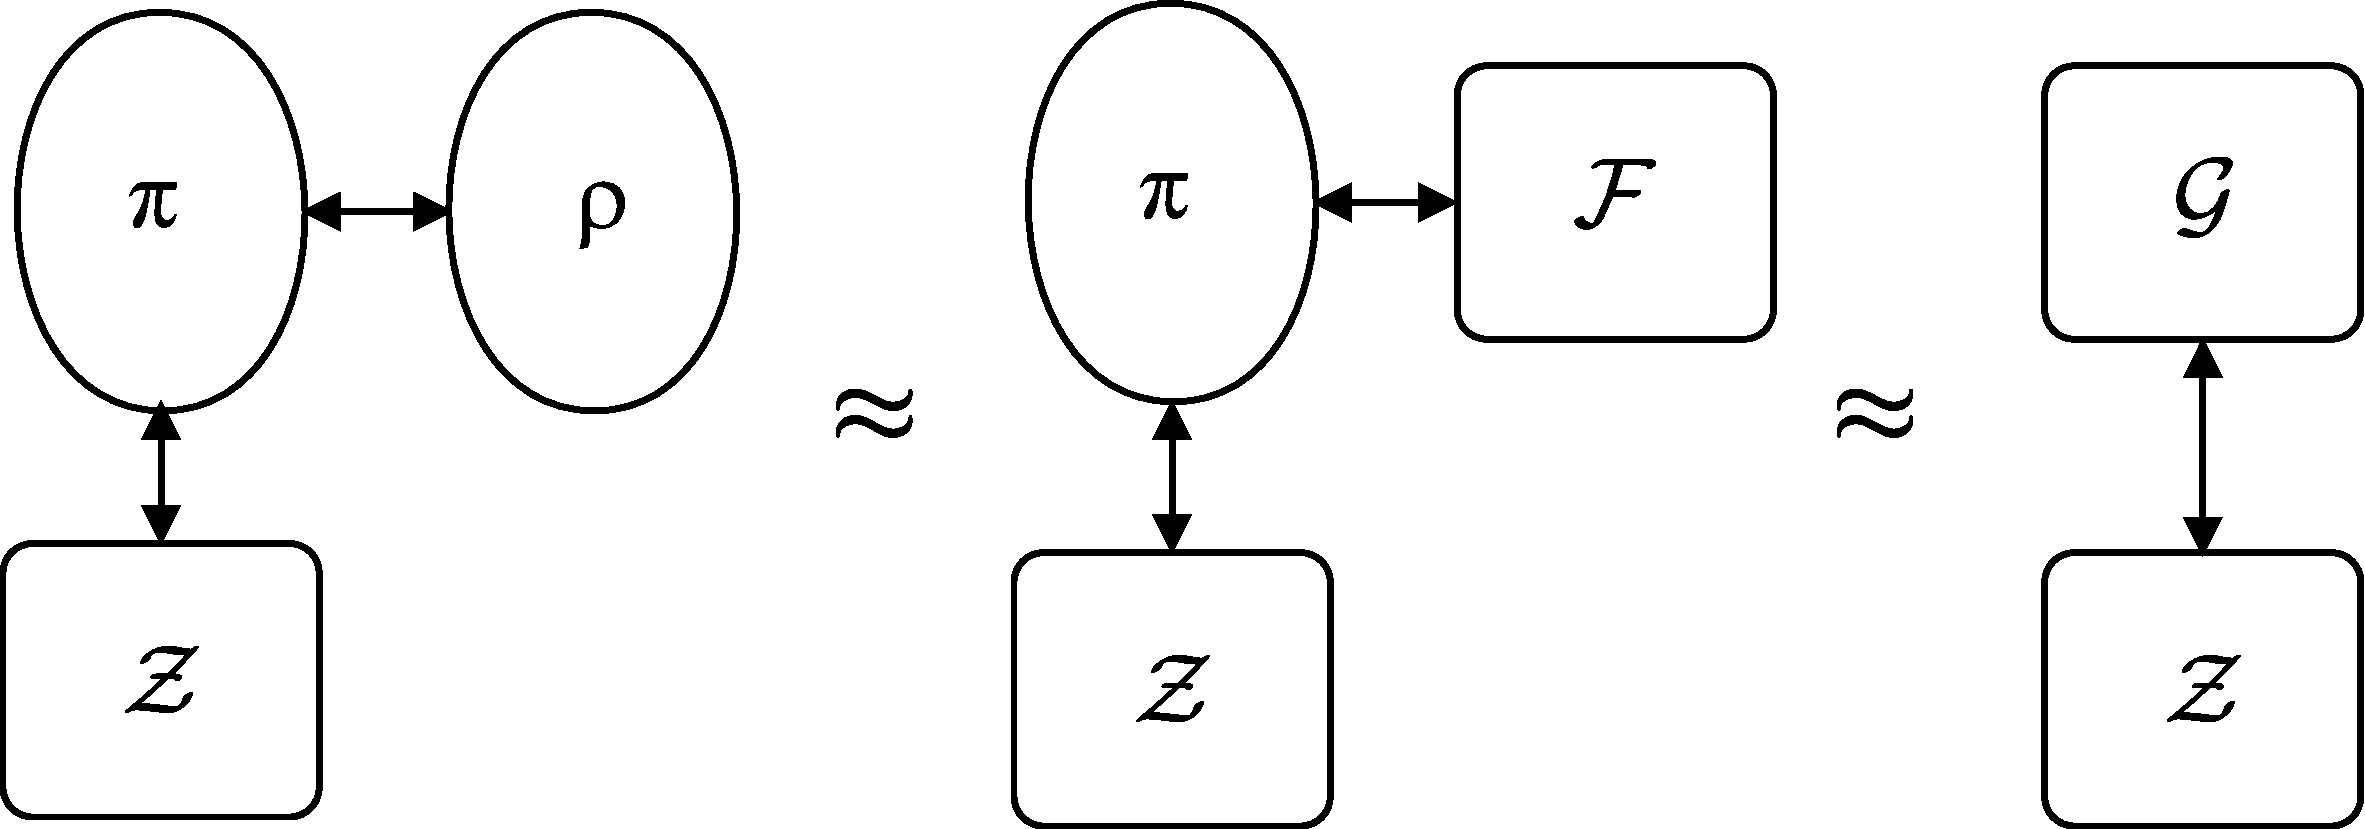
\includegraphics[width=0.7\textwidth]{figs/dolev_yao}
    \caption{Método de Dolev-Yao}
    \label{fig:dolev-yao}
\end{figure}

\section{Generalized Universal Composabillity}
Como vimos en la sección \ref{sect:uc}, para poder aplicar el teorema de composición (teorema
\ref{teo:composicion}) es necesario que el protocolo sea \textit{soubroutine respecting}.
Esto es, el protocolo y todas sus subrutinas no deben intercambiar entradas o salidas con otros
protocolos externos a la sesión. Así, el protocolo analizado es independiente de de cualquier
otro protocolo por lo que su comportamiento entrada/salida y los mensajes intercambiados en su
ejecución también son independientes. Sin embargo puede resultar poco realista en ciertas ocasiones.\\
Una escenario donde no es realista asumir que un protocolo es soubroutine respecting es donde
es necesario asumir la existencia de funcionalidades ideales sin estar UC-realizadas por algun
protocolo, lo que se conoce como una \textit{setup assumptions}. Esto es neceario cuando se desea
desarrollar un protocolo que UC-realize cierta funcionalidad, que se sabe irrealizable sin una setup
assumption. Por ejemplo consideremos el caso de ZKP, es sabido que es imposible UC-realizar
ZKP (UC-realizar la funcionalidad ideal $\mathcal{F}_{ZK}^\mathcal{R}$ para alguna relación binaria
$\mathcal{R}$) sin \textit{setup assumptions} como por ejemplo el uso de un ``string público
aleatorio'' (CRS) (del inglés \textit{common random string}) cuando la mayoría de los participantes
son corruptos. $\mathcal{F}_{CRS}$ \cite{CanKusLin06}.\\
En UC, CRS es modelado como una funcionalidad ideal $\mathcal{F}_{CRS}$ que hace público un string
aleatorio. Ciertamente $\mathcal{F}_{CRS}$ no puede ser UC-realizado por ningun protocolo, pues
en ese caso sería posible UC-realizar $\mathcal{F}_{ZK}^\mathcal{R}$. Para obtener la funcionalidad ideal
$\mathcal{F}_{CRS}$ en el mundo real es necesario que $\mathcal{F}_{CRS}$ sea ejecutado por un participante
incorruptible e inimpersonable. Esta suposición es imposible de obtener
\footnote{Basicamente hay que tener un servidor de CRS que nadie puede \textit{``hackear''}},
solo es posible usar técnicas para evitar ataques, y no son infalibles.\\
Suponiendo la existencia de $\mathcal{F}_{CRS}$, la forma de probar que un protocolo $\pi_{ZK}^\mathcal{R}$
que UC-realiza $\mathcal{F}_{ZK}^\mathcal{R}$ sería probar que $\pi_{ZK}^{R}$ en el modelo
$\mathcal{F}_{CRS}$-híbrido. Pero esta configuración tiene el inconveniente que se considera que
$\mathcal{F}_{CRS}$ es local al protocolo, por lo tanto para cada instancia de $\pi_{ZK}^\mathcal{R}$
existiría una instancia de $\mathcal{F}_{CRS}$. Más aún, también debería existir una instancia de
$\mathcal{F}_{CRS}$ para cualquier otro protocolo que lo necesite.\\
La forma correcta de modelar una setup assumption es considerar que es compartida por cada protocolo
que hace uso de ella, pero en ese caso los protcolos dejan de ser soubroutine repecting.
En \cite{Pass03} se muestra que en el caso de un $\mathcal{F}_{CRS}$ compartido
usado para UC-realizar ZKP, el protocolo perdería la propiedad de \textit{deniability} que es natural
de obtener en ZKP. Más aún, en \cite{journals/tcs/YaoYZ09} se muestra que inclusive esto puede llevar
a la perdida de la correctitud del protocolo.\\

\subsection{Ejecución de un protocolo}

\subsubsection{Ejecución en GUC}

En GUC se define una ejecución de $\pi$ donde el ambiente no esta limitado a ejecutar solo ITIs con el código del
protocolo analizado (a excepción del adverario) y SID fijo, ya que un protocolo en GUC es ejecutado con el
sITM $(\mathcal{Z}, C_{GEXEC}^{\pi, \mathcal{A}})$, donde $C_{GEXEC}^{\pi, \mathcal{A}}$ es idéntica a
$C_{EXEC}^{\pi, \mathcal{A}}$, salvo que no limita a $\mathcal{Z}$ como en UC pues permite al ambiente ejecutar
cualquier protocolo. De este modo un protocolo $\pi$
ese ejecutado cocurrentemente con otros protocolos que comparten estado con $\pi$ y por lo tanto pueden existir
ataques a un protocolo mediante la ejecución paralela de protocolos
maliciosamente correlacionados con $\pi$, lo que no es posible de modelar en UC.\\ 
Denotamos la salida de la ejecución de un protocolo $\pi$ en GUC por
$\mathrm{GEXEC}_{
    \mathcal{Z},
    \mathcal{A},
    \pi}
=
\mathrm{OUT}_{(\mathcal{Z},
              C_{GEXEC}^{\pi, \mathcal{A}})}$.\\

\begin{figure}[hp]
    \centering
    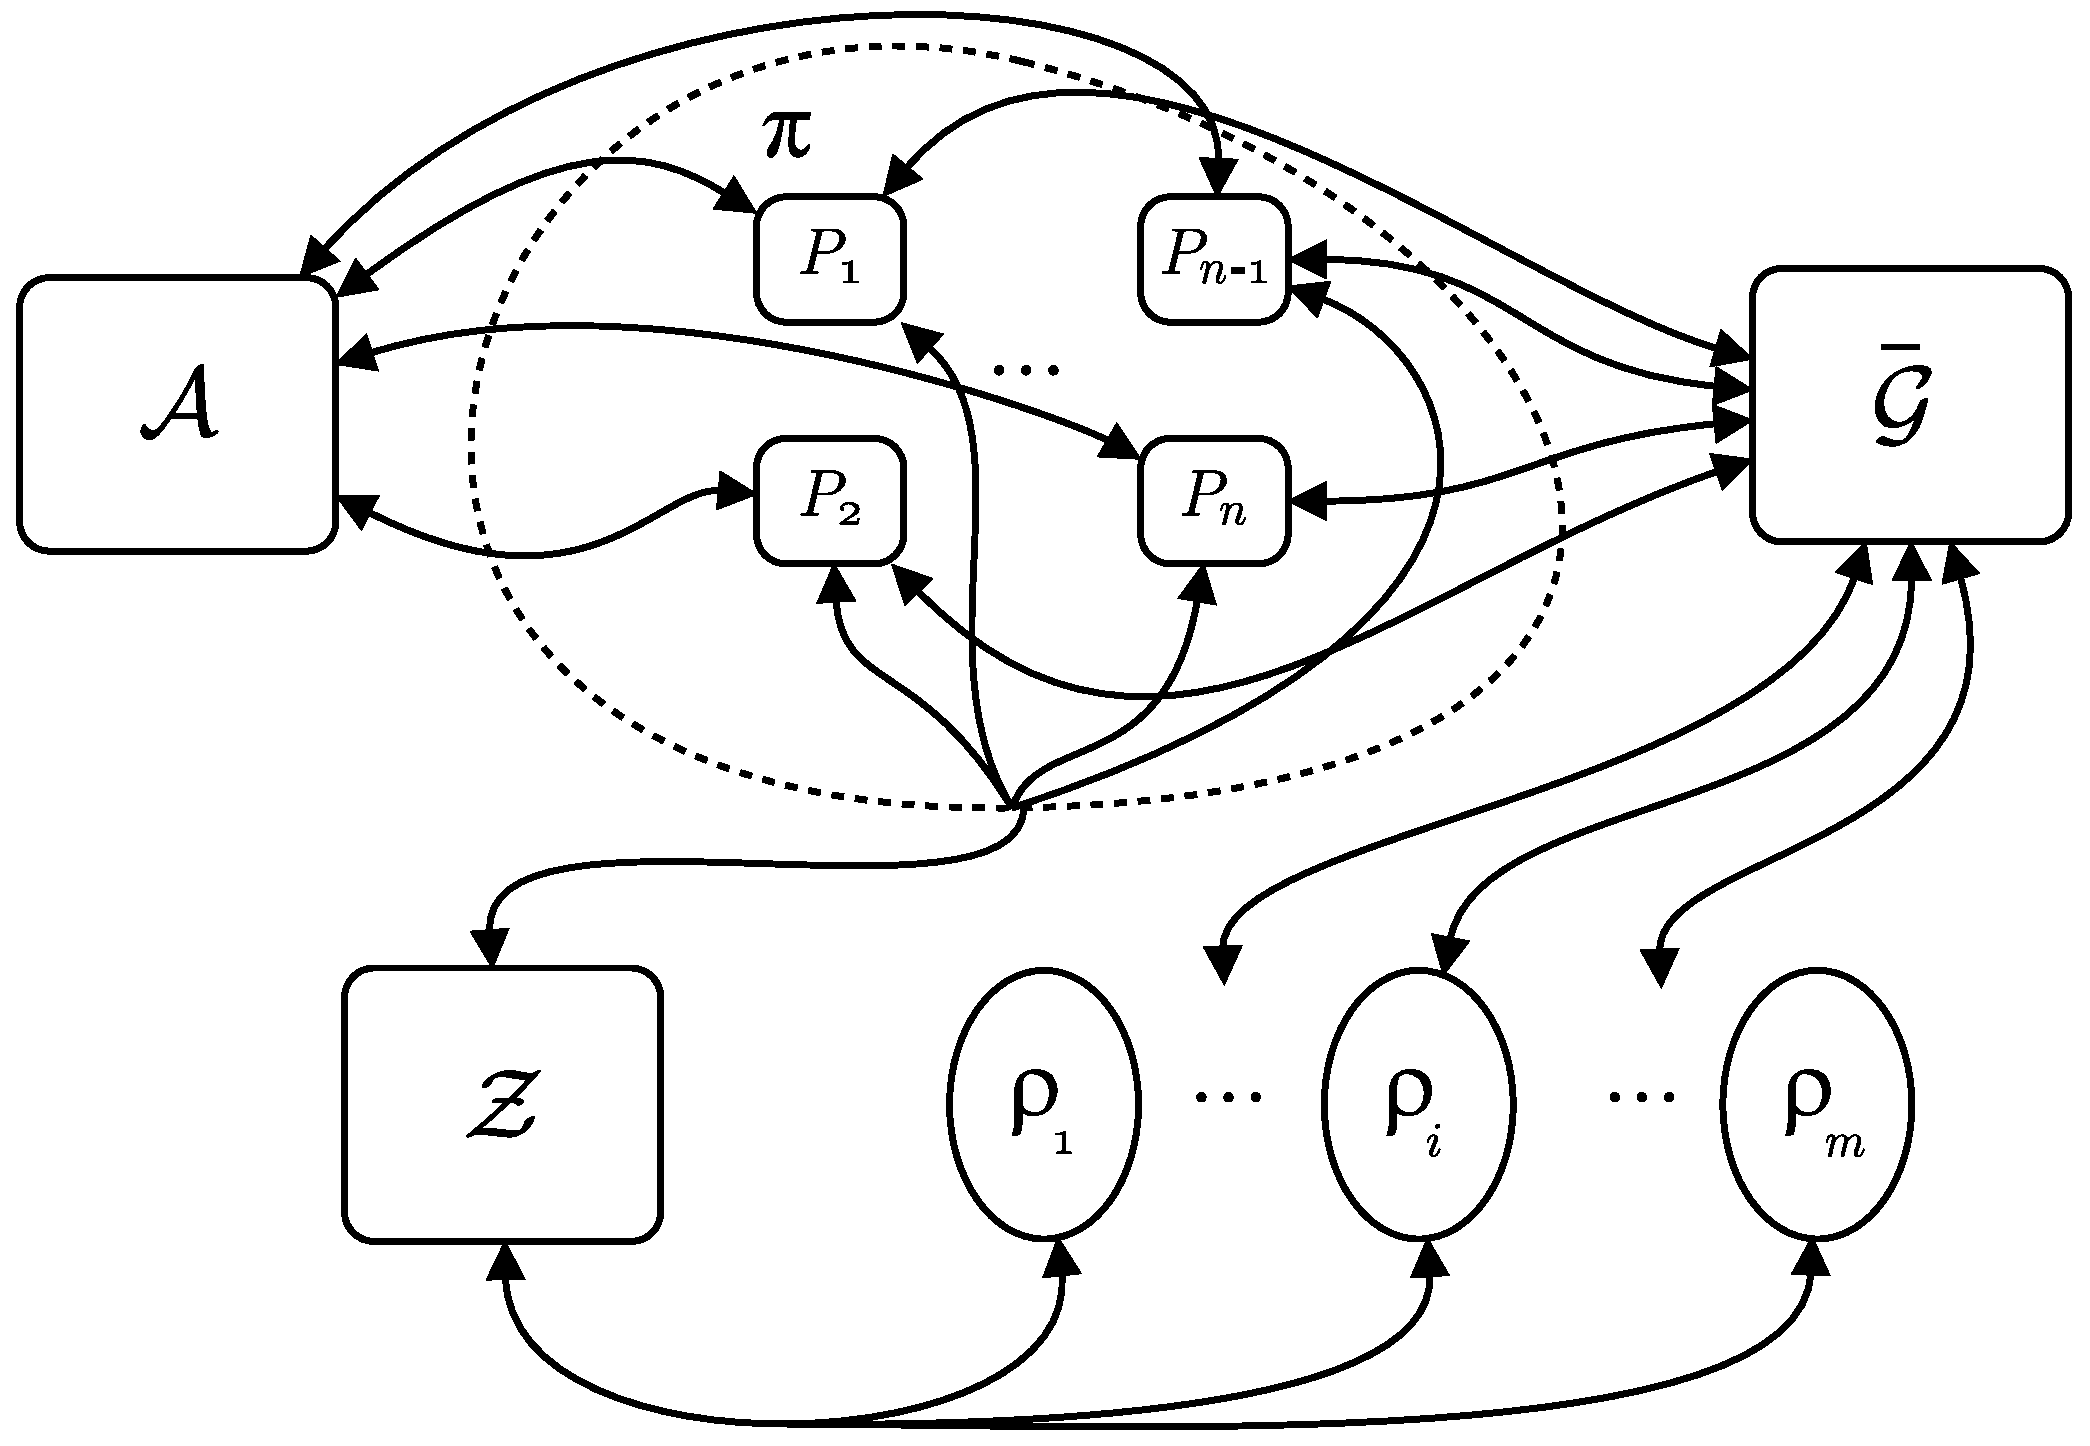
\includegraphics[width=0.7\textwidth]{figs/mundo_real_guc}
    \caption{Ejecución del protocolo $\pi$ en GUC}
    \label{fig:mundo_real_guc}
\end{figure}

Definimos la GUC-emulación como sigue.

\begin{definicion}[GUC-emulacion]
Decimos que un protocolo $\pi$ GUC-emula a otro protocolo $\rho$ si para todo ambiente $\mathcal{Z}$
y para todo adversario real $\mathcal{A}$ existe un adversario ideal $\mathcal{S}$ talque:
$$\mathrm{GEXEC}_{\mathcal{Z}, \mathcal{A}, \mathcal{\pi}}
\approx
\mathrm{GEXEC}_{\mathcal{Z}, \mathcal{A}, \mathcal{\rho}}$$
\end{definicion}

\subsubsection{Ejecución en EUC}
Un ambiente que ejecuta un conjunto arbitrario de protocolos puede resultar complejo de manipular en las
pruebas de seguridad, y resulta más cómodo trabajar con un modelo más simple aunque no menos expresivo.
En efecto es posible obtener un modelo equivalente a GUC que considera a un  solo un ambiente  con acceso
al protocolo y las interacciones de este con los demás protocolos. En este modelo, llamado EUC (del inglés
\textit{Externalized-souroutine UC}), el ambiente solo puede ejecutar una instancia del procolo más una
\textit{funcionalidad compartida}.

Las funcionalidades compartidas permiten al ambiente simular internamente la ejecución concurrente de
otros protocolos. Denotadas por la barra superior $\bar{}$, son identicas que una funcionalidad
ideal, salvo que aceptan input de cualquier ITI independiente de su SID. Su cinta de identidad contiene
el string $\#||\perp$, donde $\#$ es un SID distinto a todos los otros SID.\\

En EUC un protocolo $\pi$ puede no ser soubroutine respecting, pero sí debe ser
$\bar{\mathcal{G}}$\textit{souroutibe respecting}, donde $\bar{\mathcal{G}}$ es una funcionalidad compartida.
Al ser $\pi$ $\bar{\mathcal{G}}$-soubruotine respecting solo puede comunicarse a traves de $\bar{\mathcal{G}}$,
lo cual no resulta extraño pues en general los protocolos criptográficos comparten estado de forma encapsulable
en una funcionalidad (por ejemplo CRS o PKI).

\begin{definicion}[Protocolo $\bar{\mathcal{G}}$-soubroutine respecting]
Decimos que un protocolo es $\bar{\mathcal{G}}$-soubroutine respecting si es soubroutine respecting sin
tomar en cuenta llamadas a una funcionalidad $\bar{\mathcal{G}}$
\end{definicion}

A la salida del sITM $(\mathcal{Z}, C_{EEXEC}^{\pi, \bar{\mathcal{G}}, \mathcal{A}})$, donde
$C_{EEXEC}^{\pi, \bar{\mathcal{G}}, \mathcal{A}}$ es una función de control
como la de UC pero que adicionalmente permite al ambiente llamar a una funcionalidad compartida
$\bar{\mathcal{G}}$, la denotamos por $\mathrm{EEXEC}_{\mathcal{Z}, \mathcal{A}, \mathcal{\pi}}^{\bar{\mathcal{G}}}$
$ = \mathrm{OUT}_{(\mathcal{Z}, C_{EEXEC}^{\mathcal{A}, \pi, \bar{\mathcal{G}}})}$.\\

\begin{figure}[hp]
    \centering
    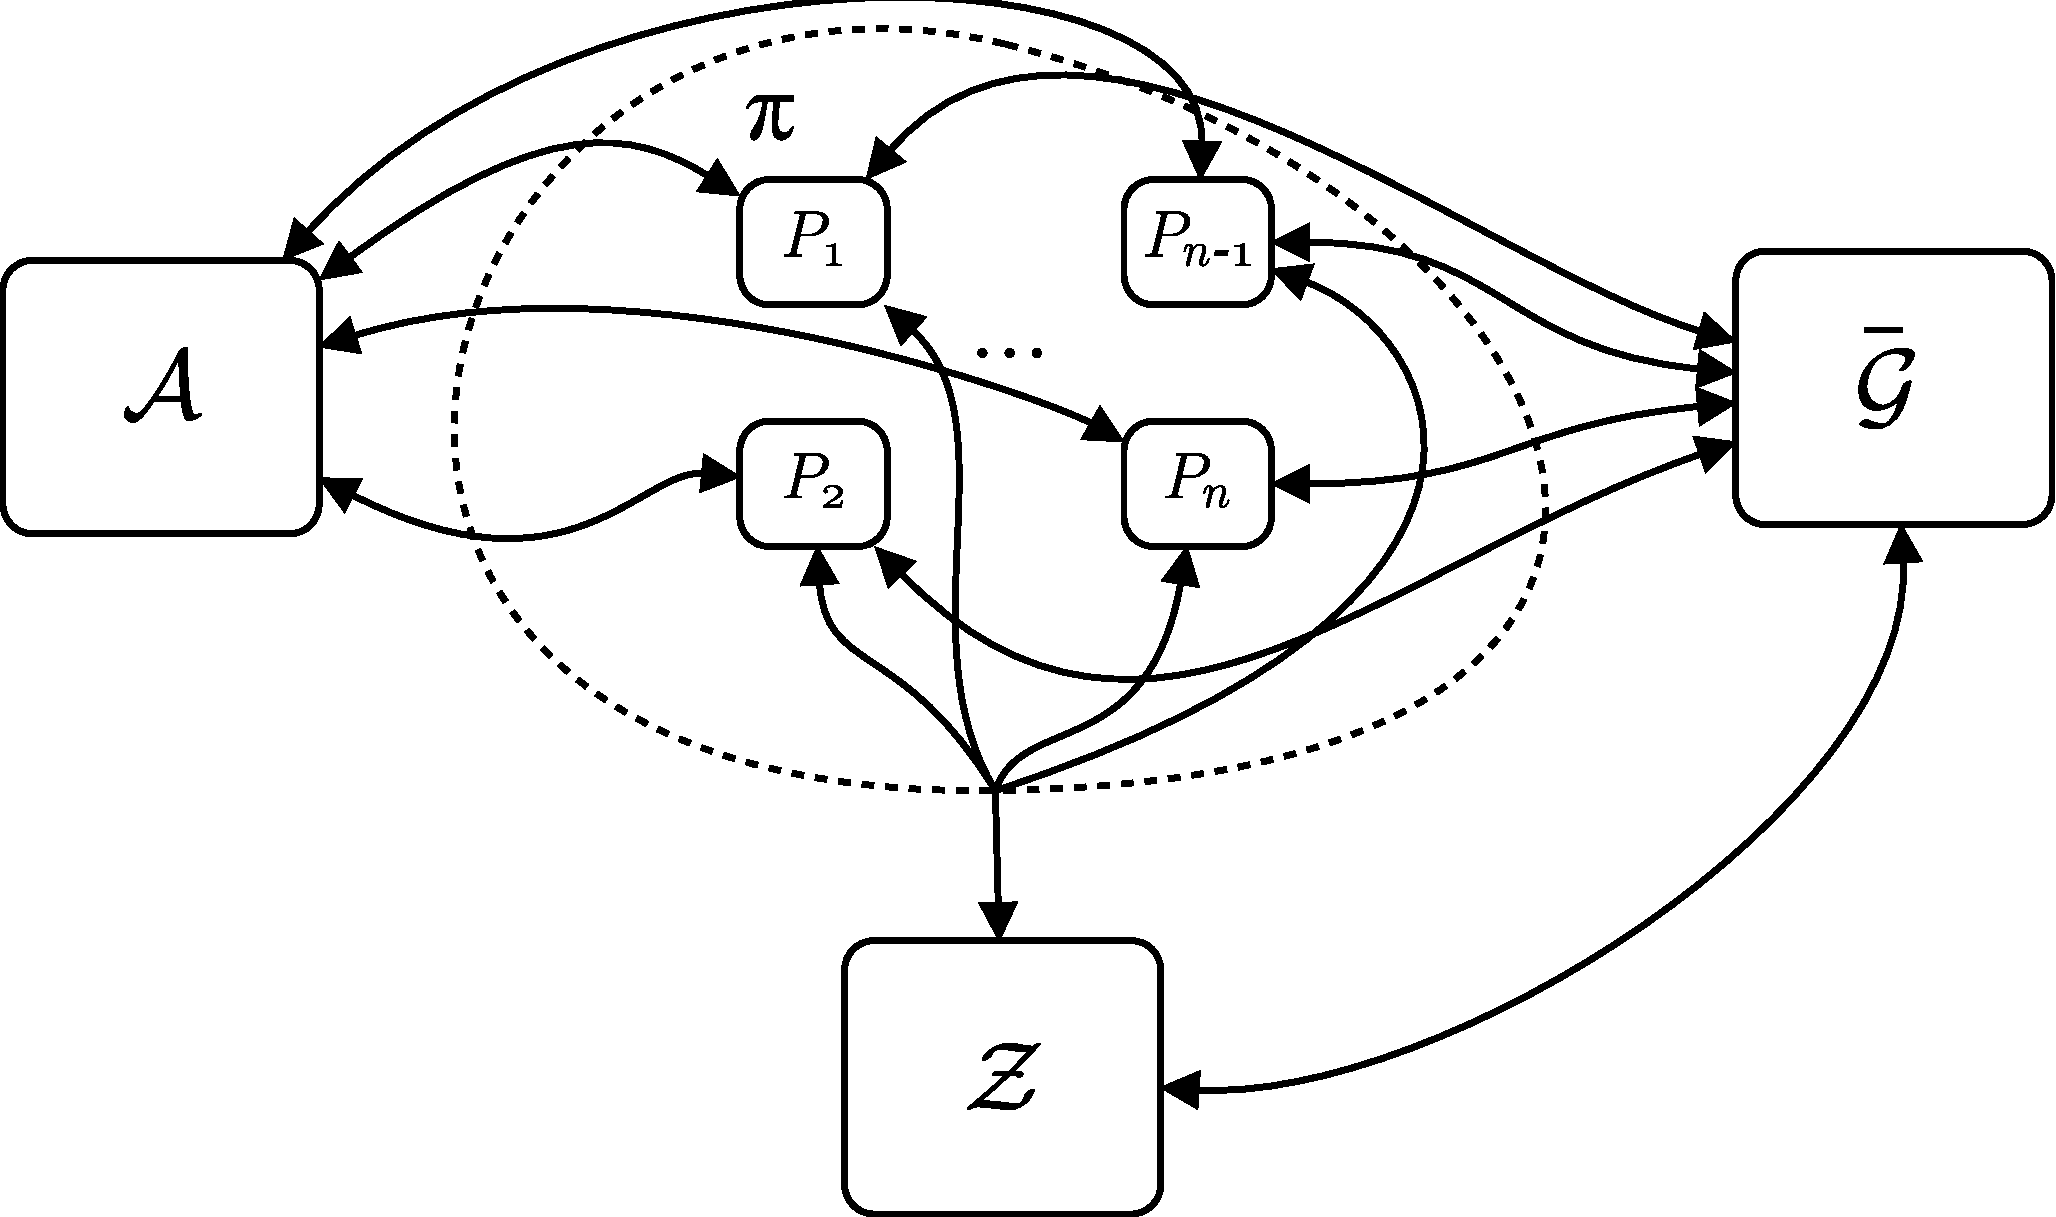
\includegraphics[width=0.7\textwidth]{figs/mundo_real_euc}
    \caption{Ejecución del protocolo $\pi$ en EUC}
    \label{fig:mundo_real_euc}
\end{figure}

Definimos la EUC-emulación como sigue.

\begin{definicion}[EUC-emulacion]
Decimos que un protocolo $\pi$ EUC-emula con funcionalidad compartida $\bar{\mathcal{G}}$ a otro protocolo
$\rho$ si para todo ambiente $\mathcal{Z}$ y para todo adversario real $\mathcal{A}$ existe un adversario
ideal $\mathcal{S}$ talque:
$$\mathrm{EEXEC}_{\mathcal{Z}, \mathcal{A}, \mathcal{\pi}}^{\bar{\mathcal{G}}}
\approx
\mathrm{EEXEC}_{\mathcal{Z}, \mathcal{S}, \mathcal{\rho}}^{\bar{\mathcal{G}}}$$
\end{definicion}

Se puede demostrar que un protocolo que EUC es solo una transformación sintáctica de UC, pues el poder
de distinción del ambiente es el mismo en ambos.

\begin{teorema}[\cite{conf/tcc/CanettiDPW07}]
Sean $\pi$ y $\rho$ dos protocolos $\bar{\mathcal{G}}$-souboutine respecting, $\pi$ GUC-emula a
$\rho$ si y solo si $\pi$ EUC-emula $\rho$.
\end{teorema}

\begin{figure}[hp]
    \centering
    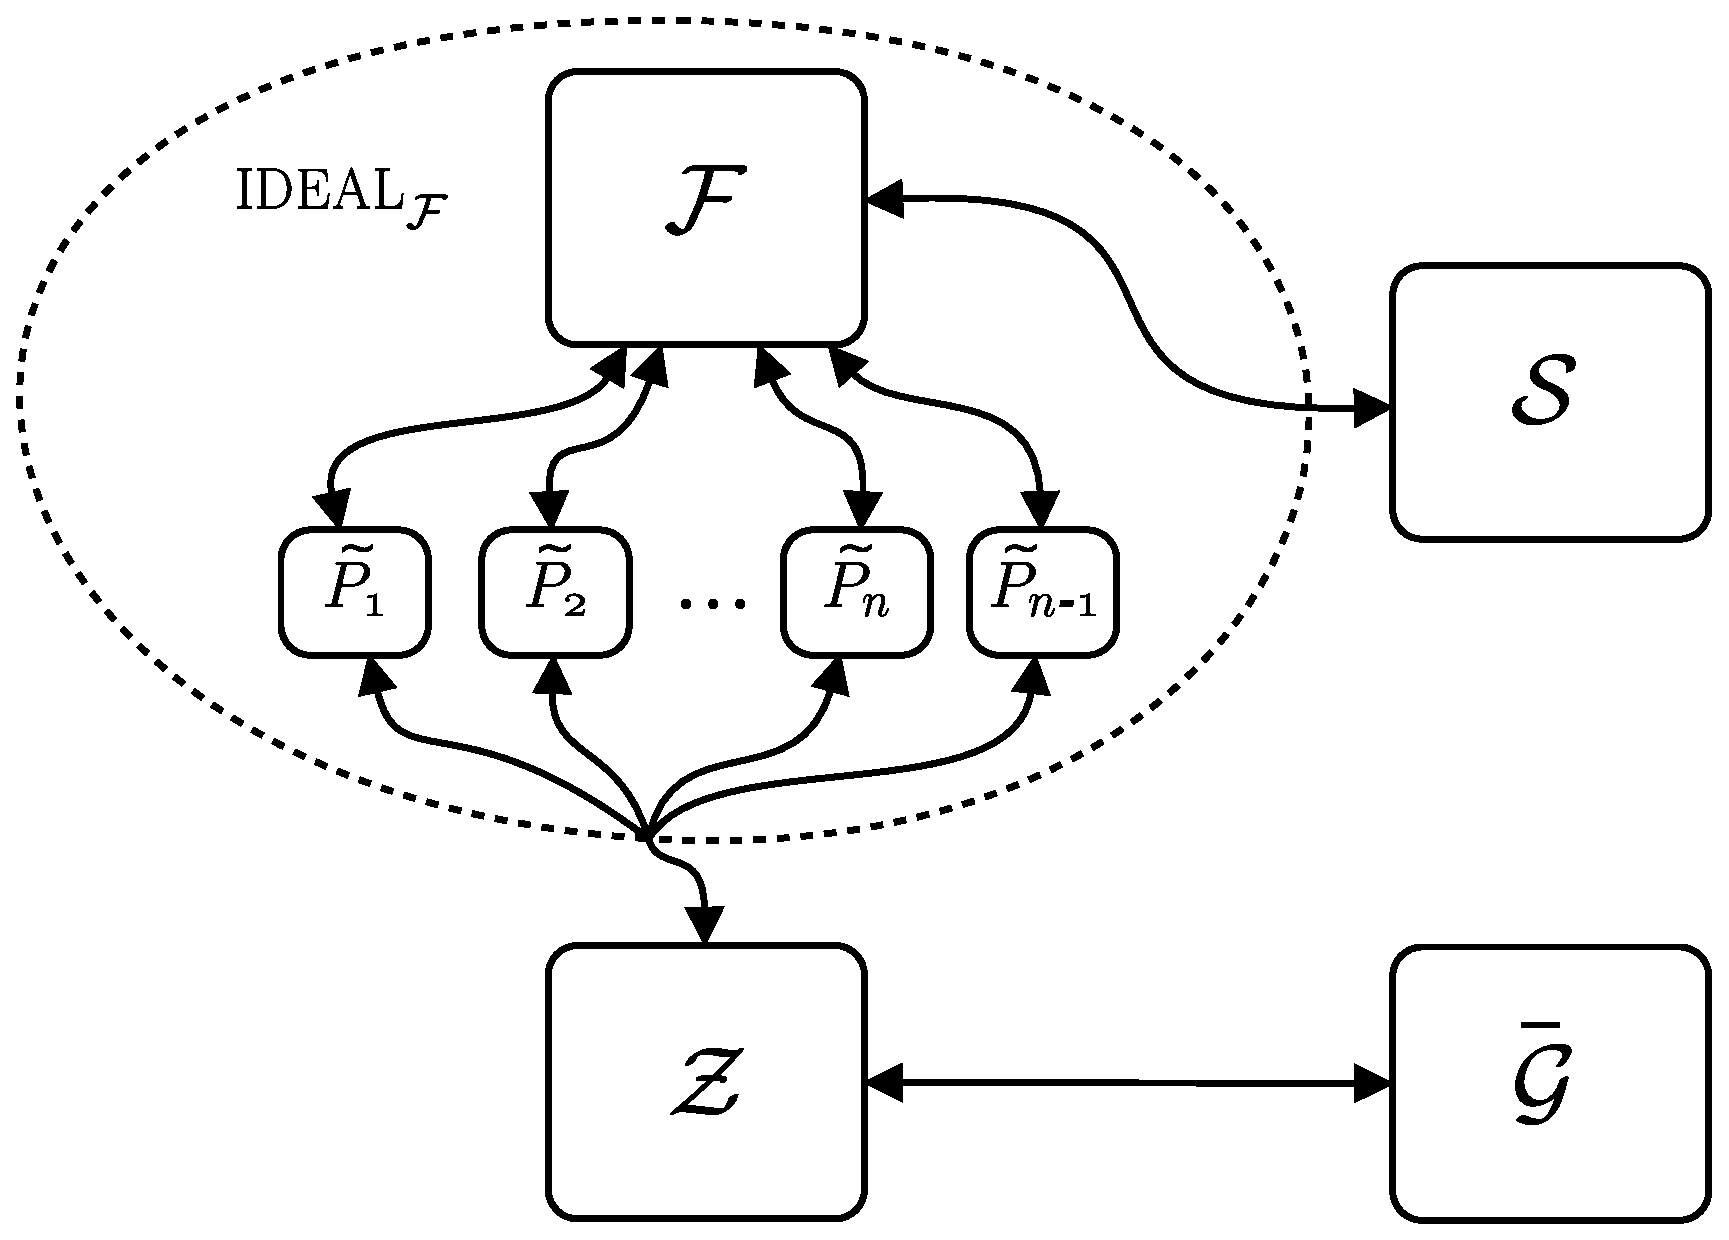
\includegraphics[width=0.7\textwidth]{figs/mundo_ideal_guc}
    \caption{Ejecución del protocolo $\textrm{IDEAL}_\mathcal{F}$ en EUC}
    \label{fig:mundo_real_euc}
\end{figure}

Intuitivamente podemos notar que todo ambiente $\mathcal{Z}$ que es ejecutado en GUC puede ser simulado por
otro ambiente EUC $\mathcal{Z'}$, que simula para $\mathcal{Z}$ todos las instancias de otros protocolos gracias
a su acceso a $\bar{\mathcal{G}}$. La otra implicancia es trivial dado que EUC es un caso especial de GUC.\\

Al igual que en UC existe un teorema de composición, que permite reemplazar protocolos reales por protocolos
ideales.

\begin{teorema}[Teorema de composición generalizado \cite{conf/tcc/CanettiDPW07}]
Sean $\pi, \rho, \phi$ protocolos tales que $\rho$ GUC-emula a $\phi$ y $\rho$ y $\phi$ son protocolos
$\bar{\mathcal{G}}$-soubroutine respecting. Entonces el protocolo $\pi^{\rho/\phi}$ GUC-emula al protoclo $\pi$.
\end{teorema}

\begin{corolario}
Sean $\pi, \rho$ protocolos y $\mathcal{F}$ una funcionalidad ideal tales que $\rho$ GUC-realiza
$\mathcal{F}$ y $\rho$ es un protocolo $\bar{\mathcal{G}}$-soubroutine respecting. Entonces el protocolo
$\pi^{\rho/\mathrm{IDEAL}_\mathcal{F}}$ GUC-emula a $\pi$.
\label{corolario:uc-realizacion}
\end{corolario}

\section{Una notación más simple para (G)UC}
Revisaremos la notacion ocupada en \cite{mnCompleto} pues simplifica el análisis de protocolos en el caso
en que el número de participantes puede estar fijo a priori. En \cite{mnCompleto} Wikstr\"om introduce una
nueva máquina a UC, llamada el modelo de comunicación. El modelo de comunicación esta a cargo de todos los
aspectos de la comunicación entre ITIs en UC. Esta notación simplifica la definición de qué puede hacer el
adversario en una ejecución, de hecho lo único que diferencia al adversario real del adversario 
ideal es el modelo de comunicación. La introducción del modelo de comunicación también hace innecesario
el uso de SIDs, pues los modelos de comunicación son locales a cada instancia de un protocolo.\\
Denotamos por $\textrm{ITM}$ el conjunto de todas las ITMs.

\begin{definicion}[grafo de ITMs]
Un grafo de ITMs en un conjunto vertices $V = \{P_1, \ldots, P_t\} \subset \textrm{ITM}$ con un conjunto
de aristas $E$ tales que $(V, E)$ es un grafo conexo, y ningún $P_i$ se puede comunicar con una máquina
fuera de $V$. Si $(P_i, P_j)\in E$ entonces se dice que $P_i$ tiene un link con $P_j$ y viceversa
\footnote{Las ITMs de esta formulación tienen tantas cintas de comunicación como vecinos.}.
Sea ITMG el conjunto de todos los grafos de ITMs.\\
Durante la ejecucion de un grafo de ITMs, a lo más un participante se encuentra activo. Un participante
activo puede desactivarse y activar a alguno de sus vecinos entregandole cierta entrada $x$, o puede
detenerse en cuyo caso la ejecución de grafo de ITMs se detiene.
\end{definicion}

El modelo de comunicación real modela una red con comunicación asíncrona, en donde el adversario
puede leer, borrar, modificar e insertar cualquier mensaje de su elección.

\begin{definicion}
Un modelo de comunicación real $\mathcal{C}$ es una ITM con un link $l_{P_i}$ a $P_i$
para $i = 1, \ldots, k$, y un link $l_\mathcal{A}$ al adversario real $\mathcal{A}$.
Su código se define como sigue.
\begin{enumerate}
  \item Si $m$ es leído en $l_s$ donde $s \in \{P_1, \ldots, P_k\}$, entonces $(s, m)$ es
        escrito en $l_\mathcal{A}$ y $mathcal{A}$ es activado.
  \item Si $(r, m)$ es leído en $l_\mathcal{A}$, donde $r \in \{P_1, \ldots, P_k\}$,
        m es escrito en $l_r$ y $P_r$ es activado.
\end{enumerate}
\end{definicion}

Por simplicidad omitimos llamar explicitamente a modelo de comunicación real.
Cuando en un protocolo del mundo real escribimos ``$P_i$ envía $m$ a $P_j$''
nos referimos a ``$P_i$ envía $(P_j, m)$ a $\mathcal{C}$''.\\
El modelo de comunicación ideal captura el hecho de que el adverasio ideal puede
decidir si y cuando enviar un mensaje desde una funcionalidad ideal a un participante,
pero no puede leer ni modificar los contenidos de la comunicación entre participantes
y la funcionalidad ideal.

\begin{definicion}
Un modelo de comunción ideal $\mathcal{C_I}$ es una ITM con un link $l_{P_i}$ a 
$P_i$ para $i = 1, \ldots, k$,
y links $l_\mathcal{F}$ y $l_\mathcal{S}$ a una funcionalidad ideal $\mathcal{F}$
y a un adversario ideal $\mathcal{S}$ respectivamente. Su código se define como sigue.
\begin{enumerate}
  \item Si un mensaje $m$ es leído en $l_s$, donde $s \in \{P_1, \ldots, P_k\}$,
        entonces $(s, m)$ es escrito en $l_\mathcal{F}$ y $\mathcal{F}$ es activada.
  \item Si un mensaje $(s, m)$ escrito en $l_\mathcal{F}$ es retornado inalterado, $m$ es
        escrito en $l_s$. Si no, cualquier string leído desde $l_\mathcal{F}$ es interpretado
        como una lista $((r_1, m_1), \ldots, (r_t, m_t))$, donde $r_i \in \{\mathcal{S},
        P_1, \ldots, P_k\}$. Por cada $m_i$ un string aleatorio $\tau_i \in \{0, 1\}^n$ es
        escogdo, y $(r_i, m_i)$ es guardado en el registro etiquetado con $(\tau_i)$. Luego
        $((r_1, |m_1|, \tau_1), \ldots, (r_t, |m_t|, \tau_t))$ is
        written on $l_\mathcal{S}$ and $\mathcal{S}$ is activated.
  \item Todo string leído desde $l_\mathcal{S}$ es interpretado como el par $(b, \tau)$, donde
        $b \in \{0, 1\}$ y $\tau$ es un string arbitrario. Si $b = 1$ y $(r_i, m_i)$
        esta guardado en el registro etiquetado con $\tau$, $m_i$ es escrito en $l_{r_i}$
        y $r_i$ es activado. Si $b = 0$ $(\mathcal{S}, \tau)$ es escrito en
        $l_\mathcal{F}$ y $\mathcal{F}$ is activada.
\end{enumerate}
\end{definicion}

El modelo ideal es equialente a una ejecución del protocolo $\textrm{IDELA}_{\mathcal{F}}$

\begin{definicion}
El modelo ideal es definido como la función $\mathcal{I}:\textrm{ITM}^2 \times
\tilde{\textrm{ITM}}^* \to \textrm{ITMG}$, donde $\mathcal{I}: (\mathcal{F}, \mathcal{S}
\tilde{P}_1, \ldots, \tilde{P}_k) \mapsto (V, E)$ viene dado por:
$$V = \{\mathcal{C_I}, \mathcal{F}, \mathcal{S}, \tilde{P}_1, \ldots, \tilde{P}_k\}$$
$$E = \{(\mathcal{S}, \mathcal{C_I}), (\mathcal{C_I}, \mathcal{F})\} \cup
\bigcup_{i = 1}^{k}\{(\tilde{P}_i, \mathcal{C_I})\}$$
\end{definicion}

Si $\tilde{\pi} = (\tilde{P}_1, \ldots, \tilde{P}_k)$, escribimos
$\mathcal{I}(\mathcal{S}, \tilde{\pi}^\mathcal{F})$ en vez de $\mathcal{I}(\mathcal{F},
\mathcal{S}, \tilde{P}_1, \ldots, \tilde{P}_k)$ para facilitar la notación.\\

El modelo real corresponde a la ejecución de un protcolo ``real'' en UC, es decir
donde los participantes se comunican a travez de la cinta de comunicación entrante.

\begin{definicion}
El modelo real es definido como la función$\mathcal{R}:\textrm{ITM}^* \to \textrm{ITMG}$,
donde $\mathcal{R}:(\mathcal{A}, P_1, \ldots, P_k) \mapsto (V, E)$ viene dado:
$$V = \{\mathcal{C}, \mathcal{A}, P_1, \ldots, P_k\}$$
$$E = \{(\mathcal{A}, \mathcal{C})\}\cup\bigcup_{i=1}^k\{(P_i, \mathcal{C})\}$$
\end{definicion}

Sea $(V, E) = \mathcal{I}(\mathcal{F}, \mathcal{S}, \tilde{P}_1, \ldots, \tilde{P}_k)$.
Entonces $\mathcal{Z}(\mathcal{I}(\mathcal{F}, \mathcal{S}, \tilde{P}_1, \ldots,
\tilde{P}_k))$ para denotar al gafo de ITMs $(V', E')$ definido por $V' = V \cup \{\mathcal{Z}\}$,
y $E' = E \cup \{(\mathcal{Z}, \mathcal{S})\} \bigcup_{i=1}^k \{(\mathcal{Z}, \tilde{P}_i)\}$.
Usamos la misma notación para el modelo real.\\

El modelo híbrido se define como sigue

\begin{definicion}
Sean
$(V, E) = \mathcal{R}(\mathcal{A}, \pi)$, $\pi = (P_1, \ldots, P_k)$.
Sean $(V_j, E_j) =
\mathcal{I}(\mathcal{S}_j,
            \tilde{\pi}^{\mathcal{F}_j}_j)$,
$\tilde{\pi}_j = (\tilde{P}_{j, 1}, \ldots, \tilde{P}_{j, k})$ para $j = 1, \ldots, t$,
y $(V_j, E_j) = \mathcal{R}(\mathcal{S}_j,\pi_j)$,
$\pi_j = (P_{j, 1}, \ldots, P_{j, k})$ for $j = t+1, \ldots, s$.\\
Denotamos por
$\mathcal{H}(
    \mathcal{A}^{
        \mathcal{S}_1,
        \ldots,
        \mathcal{S}_t},
    \pi^{
        \tilde{\pi}_1^{\mathcal{F}_1},
        \ldots,
        \tilde{\pi}_t^{\mathcal{F}_t},
        \pi_{t+1},
        \ldots,
        \pi_s})$
al modelo híbrido que se define como el grafo de ITMs $(V', E')$, donde
$$V' = V \cup \bigcup_{j=1}^t V_j \textrm{, y}$$
$$E' = 
    E
    \cup
    \bigcup_{j=1}^t E_j
    \cup
    \bigcup_{i=1}^k
        \left(
            \{(\mathcal{S}_i, \mathcal{A})\}
            \cup
            \bigcup_{j=1}^t \{(P_i, \tilde{P}_{j, i})\}
        \right)$$
De la misma forma que antes denotamos por
$\mathcal{Z}(
    \mathcal{H}(
        \mathcal{A}^{
            \mathcal{S}_1,
            \ldots,
            \mathcal{S}_t},
        \pi^{
            \tilde{\pi}_1^{\mathcal{F}_1},
            \ldots,
            \tilde{\pi}_t^{\mathcal{F}_t},
            \pi_{t+1},
            \ldots,
            \pi_s}))$
al grafo de ITMs $(V'', E'')$ definido por
$V'' = V \cup \{\mathcal{Z}\}$,
y
$E'' = 
    E'
    \cup
    \{\mathcal{Z}, \mathcal{A}\}
    \cup 
    \bigcup_{i=1}^k \{(\mathcal{Z}, P_i)\}$.
\end{definicion}

La UC-realización entonces queda como sigue.

\begin{definicion}
Un protocolo $\pi$ UC-realiza una funcionalidad ideal $\mathcal{F}$ si para todo ambiente
$\mathcal{Z}$ y para todo adversario real $\mathcal{A}$ existe un adversario ideal $\mathcal{S}$
talque
$$\mathcal{Z}(\mathcal{H}(\mathcal{A},\pi))
\approx
\mathcal{Z}(\mathcal{I}(\mathcal{S},\mathcal{F}))$$
\end{definicion}

Usando esta notación, el teorema de composición se escribe como sigue.

\begin{teorema}
Supongamos que
$\pi^{
    \tilde{\pi}_1^{\mathcal{F}_1},
    \ldots,
    \tilde{\pi}_t^{\mathcal{F}_t}}$
es un protocolo que UC-realiza a la funcionalidad ideal $\tilde{\pi}^{\mathcal{F}}$. Sea $\rho^\pi$
un prtocolo subroutine respecting. Entonces el protocolo
$\rho^{\pi/\mathcal{F}}$ en el modelo $\mathcal{F}$-híbrido UC-emula al protocolo $\rho^\pi$
\end{teorema}

Para obtener GUC hacemos la siguiente modificación. Consideremos el grafo de ITMs $(V, E)$ 
definido por
$\mathcal{H}(
    \mathcal{A}^{\mathcal{S}_1, \ldots, \mathcal{S}_t},
    \pi^{
        \tilde{\pi}_1^{\mathcal{F}_1},
        \ldots,
        \tilde{\pi}_r^{\mathcal{F}_r},
        \tilde{\pi}_{r+1}^{\bar{\mathcal{G}}_{r+1}},
        \ldots,
        \tilde{\pi}_t^{\bar{\mathcal{G}}_t},
        \pi_{t+1},
        \ldots,
        \pi_s}))$,
escribimos $\mathcal{Z}(V, E)$ para denotar el grafo de ITMs $(V'', E'')$ definido por $V'' = V \cup
\{\mathcal{Z}\}$, y $E'' = E' \cup \{\mathcal{Z}, \mathcal{A}\} \cup \bigcup_{i=1}^k
\bigcup_{j=r+1}^t \{(\mathcal{Z}, \tilde{P}_{i,j})\} \cup \bigcup_{i=1}^k \{(\mathcal{Z}, P_i)\}$.
Notese que los links $\bigcup_{i=1}^k \bigcup_{j=r+1}^t \{(\mathcal{Z}, \tilde{P}_{i,j})\}$ son todo
lo necesario para dar acceso al ambiente a las funcionalidades y compartidas y obtener GUC.

